\documentclass[11pt, a4paper]{article}
\usepackage[margin=2.4cm]{geometry}
\usepackage[T1]{fontenc}
\usepackage{lmodern}          % fontes vetoriais Type 1
\usepackage{cmap}             % ToUnicode CMap -> texto e acentos copiaveis
\usepackage[utf8]{inputenc}
\usepackage[brazil]{babel}
\usepackage{amsmath, amssymb, amsthm}
\usepackage{bm}
\usepackage{mathtools}
\usepackage{enumitem}
\usepackage{booktabs}
\usepackage{array}
\usepackage{xcolor}
\usepackage{titlesec}
\usepackage{parskip}
\usepackage{hyperref}
\usepackage{fancyhdr}
\usepackage{tcolorbox}
\usepackage{graphicx}
\tcbuselibrary{skins, breakable}

\definecolor{darkblue}{RGB}{15,55,115}
\definecolor{midblue}{RGB}{30,100,180}
\definecolor{theorybg}{RGB}{245,250,255}
\definecolor{questionbg}{RGB}{255,252,240}
\definecolor{evencolor}{RGB}{60,0,100}
\definecolor{rubricbg}{RGB}{248,246,252}
\definecolor{planbg}{RGB}{246,252,247}
\definecolor{plancolor}{RGB}{20,95,55}
\definecolor{trapbg}{RGB}{255,247,245}
\definecolor{trapcolor}{RGB}{150,35,35}

\hypersetup{colorlinks=true, linkcolor=darkblue, urlcolor=midblue,
  pdftitle={Resolucao --- Lista de Exercicios 3 --- Macroeconomia I MPE Insper},
  pdfauthor={Macroeconomia I --- MPE Insper 2026/T3}}

\setlength{\headheight}{14pt}
\pagestyle{fancy}
\fancyhf{}
\renewcommand{\headrulewidth}{0.4pt}
\fancyhead[L]{\small\textcolor{darkblue}{\textit{Macroeconomia I --- MPE Insper --- 2026/T3}}}
\fancyhead[R]{\small\textcolor{darkblue}{\thepage}}
\fancyfoot[C]{\small\textcolor{gray}{Resolução --- Lista de Exercícios 3}}

\titleformat{\section}[block]
  {\large\bfseries\color{darkblue}}{}{0pt}{}
  [\vspace{2pt}\color{darkblue}\rule{\textwidth}{1.5pt}\vspace{4pt}]

\tcbset{
  theorybox/.style={
    enhanced, breakable, colback=theorybg, colframe=darkblue,
    fonttitle=\bfseries\small, coltitle=white, boxrule=0.5pt, arc=3pt,
    left=6pt, right=6pt, top=4pt, bottom=4pt,
  },
  questionbox/.style={
    enhanced, breakable, colback=questionbg, colframe=gray!60,
    fonttitle=\bfseries\small, coltitle=black, boxrule=0.4pt, arc=2pt,
    left=6pt, right=6pt, top=4pt, bottom=4pt, title={\textit{Enunciado (original, em inglês)}},
  },
  rubricbox/.style={
    enhanced, breakable, colback=rubricbg, colframe=evencolor!70,
    fonttitle=\bfseries\small, coltitle=white, boxrule=0.4pt, arc=2pt,
    left=6pt, right=6pt, top=4pt, bottom=4pt, title={Onde estão os pontos},
  },
  planbox/.style={
    enhanced, breakable, colback=planbg, colframe=plancolor,
    fonttitle=\bfseries\small, coltitle=white, boxrule=0.5pt, arc=3pt,
    left=6pt, right=6pt, top=4pt, bottom=4pt,
  },
  trapbox/.style={
    enhanced, breakable, colback=trapbg, colframe=trapcolor!75,
    fonttitle=\bfseries\small, coltitle=white, boxrule=0.4pt, arc=2pt,
    left=6pt, right=6pt, top=4pt, bottom=4pt,
  },
}

\newcommand{\passo}[1]{\medskip\noindent\textbf{#1}\par\nobreak}
\newcommand{\intuicao}[1]{%
  \medskip\noindent\textcolor{midblue}{\textbf{Intuição econômica.}} #1\par}
\newcommand{\refbib}[1]{%
  \medskip\noindent{\small\textcolor{gray!60!black}{\textbf{Ref:} #1}}\par}
% Destaque de resposta. Precisa funcionar em texto E em modo matematico.
\newcommand{\resp}[1]{%
  \ifmmode {\color{darkblue}#1}\else\textcolor{darkblue}{\textbf{#1}}\fi}
\newcommand{\stst}{^{\ast}}
\newcommand{\Rt}{\widetilde{R}}

\setlist[enumerate,1]{label=(\alph*), itemsep=6pt, parsep=2pt, leftmargin=1.6em}
\setlist[itemize,1]{itemsep=3pt, parsep=1pt, leftmargin=1.3em, topsep=3pt}

\begin{document}

%======================================================================
\begin{center}
{\LARGE\bfseries\color{darkblue} Resolução --- Lista de Exercícios 3\par}
\vspace{4pt}
{\large MACROECONOMIA 1 --- MPE Insper --- Prof.\ Pedro G.\ Duarte\par}
\vspace{2pt}
{\normalsize 2026, 3\textordmasculine{} trimestre \quad$\cdot$\quad Entrega: 24/08/2026\par}
\vspace{2pt}
{\small Consumo e Poupança --- Kurlat (2020), cap.\ 6\par}
\end{center}
\vspace{6pt}

\begin{tcolorbox}[theorybox, title={Como ler este documento}]
\small
Duas questões, um único modelo. Tudo o que a Lista 3 pede sai do problema de dois
períodos do §6.2 do Kurlat: a Questão 1 é o modelo \emph{sem atrito} levado até a
equivalência ricardiana; a Questão 2 é o mesmo modelo com \textbf{duas coisas
quebradas} --- uma restrição de crédito e um imposto que muda preço relativo. As duas
quebras existem para derrubar exatamente a conclusão da Questão 1.

\smallskip
\textbf{Antes das resoluções vem o \hyperref[sec:plano]{Plano de leitura e preparo}}
(pp.\ \pageref{sec:plano}--\pageref{sec:fimplano}): item a item, o que ler no Kurlat, qual
ferramenta técnica o item cobra, qual é a armadilha e como saber que você já está pronto.
Se você ainda não tentou a lista, \textbf{leia só essa parte} e volte depois.

\smallskip
\textbf{Idioma.} O enunciado do professor está em inglês e é reproduzido \emph{verbatim} nas
caixas de enunciado. A resolução está em português, seguindo a convenção do projeto
(\texttt{CLAUDE.md}). Notação: a do Kurlat, com dois atalhos declarados na p.\
\pageref{sec:notacao}.

\smallskip
\textbf{Verificação.} Todo número foi calculado em Python; os scripts estão em
\texttt{Resolucao/lista3\_codigo/} e listados no Apêndice. A calibração de referência
($\beta=0{,}96$, $r=0{,}50$, $\sigma=2$) foi escolhida para que \emph{tudo} feche em número
redondo --- $\Omega=0{,}8$, $c_2/c_1=1{,}2$, $W=144$, $c_1=80$, $c_2=96$, $a=24$. Se a sua
conta não fechou redonda, provavelmente há erro de álgebra. Cada forma fechada foi
conferida contra otimização numérica direta e cada derivada contra diferenças centrais.

\smallskip
\textbf{Escopo.} Kurlat (2020), cap.\ 6 inteiro, com peso em §6.2 (pp.\ 105--116). A
Questão 1 é o Exercício 6.1 do livro com um item extra; a Questão 2 funde os Exercícios 6.5
e 6.6. Nada aqui usa horizonte infinito, incerteza ou métodos recursivos.
\end{tcolorbox}

\vspace{4pt}
\begin{center}
\small
\begin{tabular}{clcl}
\toprule
\textbf{Questão} & \textbf{Assunto} & \textbf{Pontos} & \textbf{Âncora} \\
\midrule
1 & Dois períodos com impostos; renda permanente; Ricardo & 5,0 & Kurlat §6.2 (pp.\ 105--116); Ex.\ 6.1 \\
2 & Restrição de crédito; imposto sobre a poupança       & ---  & Kurlat Ex.\ 6.5 e 6.6 (pp.\ 122--123) \\
\bottomrule
\end{tabular}\\[2pt]
{\footnotesize A Questão 1 vale 5 pontos pelo enunciado; a Questão 2 não traz pontuação
explícita --- presume-se que valha os 5 restantes.}
\end{center}

%======================================================================
\section[Plano de leitura e preparo]{Plano de leitura e preparo}
\label{sec:plano}
%======================================================================

\begin{tcolorbox}[planbox, title={A tese da lista, em uma frase}]
\small
O consumo responde a \textbf{riqueza}, não a renda corrente --- e as duas questões testam
essa frase pelos dois lados: a Questão 1 leva a lógica ao seu limite (nem o
\emph{timing} dos impostos importa) e a Questão 2 mostra as duas maneiras exatas de fazer
a frase falhar (o consumidor não consegue acessar sua riqueza; ou o imposto deixa de ser
\emph{lump-sum} e passa a mexer em preço relativo).
\end{tcolorbox}

\subsection*{1. O caminho mínimo de leitura (\textasciitilde 2h, antes de escrever qualquer coisa)}

\begin{center}
\small
\begin{tabular}{clp{7.6cm}c}
\toprule
\textbf{\#} & \textbf{Fonte} & \textbf{Por que} & \textbf{Tempo} \\
\midrule
1 & Kurlat §6.1, pp.\ 103--105
  & A visão keynesiana. Você precisa dela como \emph{contraste}: é a hipótese que a
    Questão 1(b) rejeita e que a Questão 2(c) ressuscita. & 15 min \\
2 & Kurlat §6.2, pp.\ 105--108
  & Montagem do problema, restrição intertemporal (6.2.4), equação de Euler (6.2.8).
    É a espinha das duas questões. & 30 min \\
3 & Kurlat §6.2 ``An Explicit Example'', p.\ 111
  & \textbf{A equação (6.2.9).} A Questão 1(a) é literalmente ela, com $a_0$ e impostos
    somados ao numerador. & 20 min \\
4 & Kurlat §6.2 ``The Effect of Interest Rates'', pp.\ 108--111
  & Efeito renda $\times$ substituição e a decomposição de Hicks (p.\ 110). Sem isso o
    item 1(c) é indefensável. & 25 min \\
5 & Kurlat §6.2 ``The Permanent Income Hypothesis'', pp.\ 112--113
  & O item 1(b) inteiro. & 15 min \\
6 & Kurlat §6.2 ``Taxes and Ricardian Equivalence'', pp.\ 113--116
  & Os itens 1(d) e 1(e). \textbf{Leia com atenção a p.\ 115}, que lista as hipóteses e
    diz o que o resultado \emph{não} afirma. & 25 min \\
7 & Kurlat, Exercícios 6.5 e 6.6, pp.\ 122--123
  & A Questão 2 é a fusão dos dois. Ler os enunciados originais mostra o que o professor
    cortou e o que acrescentou. & 10 min \\
\bottomrule
\end{tabular}
\end{center}

\passo{Complementares --- use só para intuição, nunca para elevar o nível técnico.}
Romer (2012, arquivo local), cap.\ 8, dá a versão rigorosa da renda permanente e da
equivalência ricardiana; Jones (2020), o capítulo de consumo, dá a versão gráfica e os
dados. Nenhum dos dois é necessário para resolver a lista.

\subsection*{2. Item a item: o que ler, o que treinar, onde se erra}

\begin{center}
\footnotesize
\renewcommand{\arraystretch}{1.25}
\begin{tabular}{@{}p{0.9cm}p{3.0cm}p{4.0cm}p{4.0cm}p{3.4cm}@{}}
\toprule
\textbf{Item} & \textbf{Ler antes} & \textbf{Ferramenta que o item cobra} &
\textbf{Armadilha que custa ponto} & \textbf{Você está pronto quando} \\
\midrule

\textbf{1(a)} & §6.2, pp.\ 105--108 e p.\ 111 (eq.\ 6.2.9)
& Eliminar $a$ para colapsar duas restrições em uma; Euler; usar
  $c_2=\theta c_1$ para substituir na RIO.
& Descontar $c_2$ \emph{multiplicando} por $(1+r)$; esquecer $a_0$; achar que $a_0$
  reaparece no período 2.
& Você escreve a RIO e a Euler de memória em 1 minuto e chega em (6.2.9) sem consultar. \\

\textbf{1(b)} & §6.2, pp.\ 112--113 (renda permanente); §6.1 como contraste
& Derivar a forma fechada em $y_2$ e comparar com a derivada em $y_1$.
& Responder ``sobe'' sem quantificar; esquecer de dizer o que acontece com a
  \emph{poupança}; misturar com a função consumo keynesiana.
& Você explica em palavras por que a razão entre as duas propensões é exatamente
  $1/(1+r)$. \\

\textbf{1(c)} & §6.2, pp.\ 108--111, com atenção à p.\ 110 (Hicks)
& Derivar $\Omega$ em relação a $r$; escrever o resultado em elasticidade.
& Trocar $\sigma$ por EIS $=1/\sigma$; afirmar que juro maior sempre eleva a poupança;
  não perceber que $y_2=0$ foi imposto justamente para \emph{matar} o efeito-riqueza da
  renda futura.
& Você desenha a rotação e as três setas de cabeça e diz o sinal para
  $\sigma=0{,}5$, $1$ e $2$ sem calcular nada. \\

\textbf{1(d)} & §6.2, pp.\ 113--116
& Derivadas de $W$ em $\tau_1$ e $\tau_2$; notar que $\theta$ \emph{não} depende de
  imposto nenhum.
& Dizer que um imposto hoje derruba $c_1$ na razão de $1{:}1$; errar o sinal de
  $\partial a/\partial\tau_2$ (ele é \textbf{positivo}).
& Você preenche a tabela dos seis sinais sem fazer conta. \\

\textbf{1(e)} & §6.2, pp.\ 113--116, sobretudo a p.\ 115
& Mostrar que $\tau_1,\tau_2$ entram só via $\tau_1+\frac{\tau_2}{1+r}$; aplicar o
  experimento $d\tau_1=-1$, $d\tau_2=+(1+r)$.
& Concluir ``logo política fiscal não faz nada'' --- Kurlat alerta contra isso
  explicitamente na p.\ 115; esquecer que a \emph{poupança} muda (em $+1$).
& Você lista as quatro hipóteses da equivalência e aponta qual delas a Questão 2
  quebra. \\

\textbf{2(a)} & Kurlat Ex.\ 6.5 (p.\ 122); §6.2 sobre a reta orçamentária
& Ler a desigualdade como teto de endividamento; identificar o limite natural
  $b\le\frac{y_2-\tau_2}{1+r}$.
& Dizer que $b$ é ``a poupança''; confundir $a\ge-b$ com $a\ge0$; esquecer que a
  restrição não elimina a possibilidade de poupar. & Você diz o que $b=0$ e
  $b=\infty$ significam em uma frase cada. \\

\textbf{2(b)} & O próprio $a\stst$ irrestrito do item 1(a)
& Ler o sinal da fórmula de $a\stst$: o que a torna mais negativa?
& Dar exemplos que não movem $a\stst$ (ex.: ``o consumidor é pobre'' --- pobre nos
  \emph{dois} períodos não quer tomar emprestado).
& Cada exemplo seu aponta para um parâmetro específico da fórmula. \\

\textbf{2(c)} & Kurlat Ex.\ 6.5, dica do enunciado; \texttt{rules/04}, seção ``Extensões''
& KKT / análise de dois casos; achar o limiar; verificar qual caso vale.
& Impor a Euler com \emph{igualdade} no caso ativo --- ali ela vale como
  \textbf{desigualdade}; parar antes de decidir qual caso vale.
& Você enuncia o teste ``$c_1^u>y_1-\tau_1+b$?'' sem hesitar. \\

\textbf{2(d)} & Kurlat Ex.\ 6.6 (pp.\ 122--123); §6.2 sobre a inclinação da reta
& Trocar $(1+r)$ por $(1+r-\tau_2)$ \emph{dentro da Euler}; argumento ``era factível e
  não foi escolhido''.
& Comparar os dois impostos com receitas diferentes (a comparação exige
  $T=\tau_2 a^S$); afirmar que o imposto necessariamente reduz a poupança --- o
  \textbf{sinal disso depende de $\sigma$}, o da razão $c_2/c_1$ não.
& Você diz, sem desenhar, qual imposto \emph{translada} e qual \emph{gira} a reta, e em
  torno de que ponto. \\
\bottomrule
\end{tabular}
\end{center}

\subsection*{3. Cronograma sugerido --- três sessões}

\begin{center}
\small
\begin{tabular}{@{}llp{9.4cm}@{}}
\toprule
\textbf{Sessão} & \textbf{Duração} & \textbf{O que fazer} \\
\midrule
\textbf{I --- Ferramenta}
& \textasciitilde 2h
& Leitura 1--3 do caminho mínimo. Ao final, feche o livro e derive a eq.\ (6.2.9)
  do zero em papel em branco. Só depois faça o item \textbf{1(a)}. Se travar, o
  problema é a leitura 2, não o item. \\
\textbf{II --- Estática comparativa}
& \textasciitilde 2h30
& Leituras 4--6. Faça \textbf{1(b)}, \textbf{1(c)}, \textbf{1(d)} e \textbf{1(e)} em
  sequência --- eles são quatro derivadas da \emph{mesma} fórmula. Desenhe o gráfico
  de 1(c) grande, à mão, antes de derivar qualquer coisa. \\
\textbf{III --- As duas quebras}
& \textasciitilde 2h
& Leitura 7. Faça a Questão 2 inteira. Ao terminar 2(c), volte a 1(e) e responda:
  \emph{o que exatamente da hipótese ricardiana morreu aqui?} Ao terminar 2(d),
  responda: \emph{e aqui, o que morreu?} As duas respostas são diferentes, e essa é a
  lista toda. \\
\bottomrule
\end{tabular}
\end{center}

\begin{tcolorbox}[trapbox, title={As cinco confusões que mais custam nota nesta lista}]
\small
\begin{enumerate}[label=\arabic*.]
\item \textbf{$\sigma$ contra $1/\sigma$.} $\sigma$ é a aversão relativa ao risco;
$1/\sigma$ é a elasticidade de substituição intertemporal (EIS). O item 1(c) inteiro
depende de não trocar os dois.
\item \textbf{Fator contra taxa de desconto.} $\beta$ é fator; $\rho$, com
$\beta=\frac{1}{1+\rho}$, é taxa. Um sobe quando o outro desce.
\item \textbf{Imposto \emph{lump-sum} contra imposto distorcivo.} O primeiro só desloca
$W$; o segundo muda o preço relativo. Toda a diferença entre 1(e) e 2(d) mora aqui.
\item \textbf{Euler como igualdade sempre.} Com a restrição de crédito ativa ela vale
como $u'(c_1)>\beta(1+r)u'(c_2)$. Escrevê-la com $=$ no caso ativo invalida 2(c).
\item \textbf{``Ricardo diz que política fiscal não importa''.} Não diz. Diz que o
\emph{timing} de impostos \emph{lump-sum} de mesmo valor presente não importa. Gasto do
governo, impostos distorcivos e restrição de crédito continuam importando --- é
literalmente o que a Questão 2 demonstra.
\end{enumerate}
\end{tcolorbox}

\begin{tcolorbox}[planbox, title={O que você precisa saber de cor ao entrar na prova}]
\small
Quatro objetos. Nada mais desta lista é decorável, e nada menos é suficiente.
\begin{align*}
\text{\textbf{1. Riqueza:}}\quad & W = a_0 + (y_1-\tau_1) + \frac{y_2-\tau_2}{1+r} \\[2pt]
\text{\textbf{2. Euler:}}\quad & u'(c_1) = \beta(1+r)\,u'(c_2)
  \ \Longrightarrow\ \frac{c_2}{c_1} = [\beta(1+r)]^{1/\sigma} \equiv \theta \\[2pt]
\text{\textbf{3. Forma fechada:}}\quad & c_1 = \frac{W}{1+\Omega},
  \qquad \Omega \equiv \beta^{1/\sigma}(1+r)^{\frac{1}{\sigma}-1} \\[2pt]
\text{\textbf{4. Geometria:}}\quad & \text{\emph{lump-sum} translada a reta;
  juro e imposto sobre poupança \textbf{giram} a reta em torno da dotação.}
\end{align*}
Da 3 saem 1(a), 1(b), 1(d) e 1(e); da 2 saem 1(c) e 2(d); da 4 sai todo o argumento
gráfico. Note ainda a ponte $\theta=(1+r)\Omega$, que economiza metade das contas.
\end{tcolorbox}
\label{sec:fimplano}

%======================================================================
\section[Notação e o núcleo comum]{Notação e o núcleo comum às duas questões}
\label{sec:notacao}
%======================================================================

\passo{Dois atalhos, usados o documento inteiro.}
O enunciado não os nomeia, mas eles aparecem em toda conta a partir daqui:

\begin{center}
\begin{tabular}{@{}cl@{}}
\toprule
$\displaystyle \Omega \equiv \beta^{1/\sigma}(1+r)^{\frac{1}{\sigma}-1}$
  & é o \emph{denominador menos um} da eq.\ (6.2.9) do Kurlat. \\[6pt]
$\displaystyle \theta \equiv [\beta(1+r)]^{1/\sigma} = \frac{c_2}{c_1}$
  & é a razão de consumos que a equação de Euler impõe. \\
\bottomrule
\end{tabular}
\end{center}

Os dois estão ligados por $\theta = (1+r)\,\Omega$, e a propensão marginal a consumir a
riqueza é $\mathrm{PMgC} \equiv \dfrac{1}{1+\Omega} \in (0,1)$.

\passo{A calibração de referência.}
Sempre que aparecer um número neste documento, ele vem de
$\beta=0{,}96$, $r=0{,}50$, $\sigma=2$. Essa escolha não é inocente:
$$\Omega = \sqrt{\frac{\beta}{1+r}} = \sqrt{\frac{0{,}96}{1{,}5}} = \sqrt{0{,}64} = \resp{0{,}8},
\qquad
\theta = \sqrt{\beta(1+r)} = \sqrt{1{,}44} = \resp{1{,}2},
\qquad
\mathrm{PMgC} = \frac{1}{1{,}8} = \resp{\tfrac{5}{9}}$$
Um período é ``metade de uma vida adulta'', então $r=50\%$ acumulado ao longo de umas duas
décadas é perfeitamente razoável --- e faz todo número fechar redondo.

%======================================================================
\section[Questão 1 --- Dois períodos com impostos]{Questão 1 \quad Dois períodos com impostos: da Euler a Ricardo \hfill \normalsize (5 pontos)}
%======================================================================

\begin{tcolorbox}[questionbox]
\small
Suppose a household solves the following two-period consumption-savings problem with taxes:
$$\max_{\{c_1,a,c_2\}} u(c_1)+\beta u(c_2)
\qquad \text{s.t.} \quad
\begin{aligned}
c_1 + a &= a_0 + y_1 - \tau_1 \\
c_2 &= y_2 - \tau_2 + (1+r)a
\end{aligned}$$
with $u(c)=\frac{c^{1-\sigma}}{1-\sigma}$ for $\sigma\neq1$ and $u(c)=\ln c$ for
$\sigma=1$, where: $c_1$, $y_1$ and $\tau_1$ are consumption, income and taxes at period 1,
$c_2$, $y_2$ and $\tau_2$ are consumption, income and taxes at period 2, $a_0$ is an
exogenous initial level of wealth, and $r$ is the real interest rate at which the household
can freely borrow and lend. Assume $\beta\in(0,1)$, $\sigma>0$ and $r>-1$.

\smallskip
\textbf{(a)} Solve for the household's choice of $c_1$, $c_2$ and $a$ in closed form.
\textbf{(b)} How does $c_1$ depend on $y_2$? How can we relate this to households suddenly
becoming more optimistic about the future?
\textbf{(c)} Suppose $y_2=\tau_1=\tau_2=0$ and compute $\frac{\partial c_1}{\partial r}$.
How does the answer depend on $\sigma$? Interpret the answer.
\emph{Hint: Think about what $\sigma$ means for the relative importance of income and
substitution effects.}
\textbf{(d)} Return to the general case and consider the effects of taxation. Show how
consumption in both periods and savings between period one and two are affected by
government taxation.
\textbf{(e)} Show that $\tau_1$ and $\tau_2$ affect consumption only through the present
value of $\tau_1+\frac{\tau_2}{1+r}$. Using this, describe what happens to $c_1$, $c_2$ and
$a$ if the government cuts $\tau_1$ by one unit and raises $\tau_2$ by $1+r$. Does the
timing of the taxation matter for households' consumption?
\end{tcolorbox}

%---------------------------------------------------------------- (a)
\subsection*{(a) Forma fechada para $c_1$, $c_2$ e $a$}

\passo{Passo 1 --- colapsar duas restrições em uma.}
As duas restrições período a período contêm a mesma incógnita $a$. Isole-a na segunda,
$$a = \frac{c_2 - y_2 + \tau_2}{1+r},$$
e substitua na primeira. O ativo desaparece e sobra a \textbf{restrição orçamentária
intertemporal} (RIO):
$$\boxed{\;c_1 + \frac{c_2}{1+r} \;=\; \underbrace{a_0 + (y_1-\tau_1)
+ \frac{y_2-\tau_2}{1+r}}_{\textstyle \equiv\, W}\;}$$
Duas leituras importam aqui. Primeira: o preço relativo do consumo futuro é
$\frac{1}{1+r}$ --- é isso que uma mudança de $r$ vai mexer, e nada mais.
Segunda: \textbf{a renda entra apenas por $W$}, e sempre em valor presente. Toda a
Questão 1 é consequência desses dois fatos.

\passo{Passo 2 --- a condição de primeira ordem.}
Maximizar $u(c_1)+\beta u(c_2)$ sujeito à RIO. Com o Lagrangiano
$\mathcal{L}=u(c_1)+\beta u(c_2)+\lambda\!\left[W-c_1-\frac{c_2}{1+r}\right]$:
$$u'(c_1)=\lambda, \qquad \beta u'(c_2)=\frac{\lambda}{1+r}
\quad\Longrightarrow\quad
\boxed{\;u'(c_1)=\beta(1+r)\,u'(c_2)\;}$$
que é a \textbf{equação de Euler}, eq.\ (6.2.8) do Kurlat. Como $u$ é estritamente côncava
($u''=-\sigma c^{-\sigma-1}<0$) e o conjunto orçamentário é convexo, a CPO é necessária
\emph{e} suficiente: a solução interior é única.

\passo{Passo 3 --- explorar a forma CRRA.}
Com $u'(c)=c^{-\sigma}$ --- válido inclusive no caso log, pois $\frac{d}{dc}\ln c = c^{-1}$
--- a Euler vira $c_1^{-\sigma}=\beta(1+r)c_2^{-\sigma}$, ou seja
$$\frac{c_2}{c_1}=[\beta(1+r)]^{1/\sigma}\equiv\theta .$$
Repare no que isso significa: \textbf{a razão entre os consumos não depende de renda, de
riqueza nem de imposto} --- só de $\beta$, $r$ e $\sigma$. É a homoteticidade do CRRA, e ela
faz sozinha metade do trabalho dos itens (d) e (e).

\passo{Passo 4 --- fechar.}
Substituindo $c_2=\theta c_1$ na RIO e usando $\frac{\theta}{1+r}=\Omega$:
$$c_1\left(1+\frac{\theta}{1+r}\right)=W
\quad\Longrightarrow\quad
c_1\,(1+\Omega)=W$$

\begin{tcolorbox}[theorybox, title={Resposta do item (a)}]
$$\resp{c_1\stst = \frac{W}{1+\Omega}
= \frac{a_0+(y_1-\tau_1)+\dfrac{y_2-\tau_2}{1+r}}
       {1+\beta^{1/\sigma}(1+r)^{\frac{1}{\sigma}-1}}}$$
$$\resp{c_2\stst = [\beta(1+r)]^{1/\sigma}\,c_1\stst
= \frac{[\beta(1+r)]^{1/\sigma}\,W}{1+\Omega}}$$
$$\resp{a\stst = a_0+y_1-\tau_1-c_1\stst
= \underbrace{\frac{\Omega}{1+\Omega}}_{1-\mathrm{PMgC}}(a_0+y_1-\tau_1)
 \;-\; \underbrace{\frac{1}{1+\Omega}}_{\mathrm{PMgC}}\cdot\frac{y_2-\tau_2}{1+r}}$$
\end{tcolorbox}

\passo{Duas verificações.}
\emph{(i) Caso log.} Com $\sigma=1$, $\Omega=\beta$ e $\theta=\beta(1+r)$, logo
$c_1=\frac{W}{1+\beta}$ --- e $c_1$ deixa de depender de $r$ dado $W$. Guarde isso: é
exatamente o item (c).
\emph{(ii) Suavização perfeita.} Se $\beta(1+r)=1$, então $\theta=1$ e $c_1=c_2$ para
\textbf{qualquer} $\sigma$. Impaciência e juro se cancelam e o consumidor achata o perfil.

\passo{A forma do $a\stst$ merece leitura.}
Note a estrutura da terceira linha: a poupança é uma \emph{diferença} entre a fração não
consumida dos recursos disponíveis hoje e o valor presente dos recursos de amanhã. Um
consumidor com muita renda futura e pouca renda presente tem $a\stst<0$ --- ele toma
emprestado. Essa é a expressão que a Questão 2(b) vai interrogar.

\passo{Números da calibração de referência.}
Com $\beta=0{,}96$, $r=0{,}5$, $\sigma=2$, $a_0=10$, $y_1=100$, $y_2=69$, $\tau_1=6$,
$\tau_2=9$:
$$W = 10+94+\frac{60}{1{,}5}=\resp{144},\qquad
c_1\stst=\frac{144}{1{,}8}=\resp{80},\qquad
c_2\stst=1{,}2\times 80=\resp{96},\qquad
a\stst=104-80=\resp{24}$$
Confere pela restrição do período 2: $60+1{,}5\times24 = 96$. \checkmark

\refbib{Kurlat (2020), §6.2 (pp.\ 105--108) para a RIO (6.2.4) e a Euler (6.2.8);
``An Explicit Example'' (p.\ 111) para a eq.\ (6.2.9), que é este item sem $a_0$ e sem
impostos. Observação de notação: o livro usa $u(c)=\frac{c^{1-\sigma}}{1-\sigma}$ e as
regras do projeto, $\frac{c^{1-\sigma}-1}{1-\sigma}$; diferem por uma constante aditiva e
têm a \emph{mesma} $u'$, logo a mesma solução.}

\begin{tcolorbox}[rubricbox]
\small
\begin{itemize}[topsep=2pt]
\item Não derivar a RIO e trabalhar com as duas restrições soltas: mesmo chegando ao
      resultado, máx.\ 0,7 do item --- a RIO \emph{é} o conteúdo.
\item Euler correta mas parar antes da forma fechada: máx.\ 0,5 (o enunciado diz
      ``in closed form'', e o Kurlat define o termo em nota de rodapé).
\item Esquecer $a_0$ em $W$: $-0{,}3$, e contamina (d) e (e).
\item Não dar $a\stst$ (só $c_1$ e $c_2$): $-0{,}3$.
\end{itemize}
\textbf{Bônus de completude:} observar que $\theta$ não depende de renda nem de imposto,
e sinalizar que isso já resolve parte de (d) e (e).
\end{tcolorbox}

%---------------------------------------------------------------- (b)
\subsection*{(b) Como $c_1$ depende de $y_2$ --- e o que é ``otimismo''}

\passo{A derivada.}
$y_2$ entra na solução do item (a) apenas dentro de $W$, e lá com peso $\frac{1}{1+r}$:
$$\frac{\partial c_1\stst}{\partial y_2}
=\frac{1}{1+\Omega}\cdot\frac{\partial W}{\partial y_2}
=\resp{\frac{1}{(1+\Omega)(1+r)}=\frac{\mathrm{PMgC}}{1+r}}\;>\;0$$

Três propriedades, e cada uma vale um pedaço da resposta:

\begin{center}
\small
\begin{tabular}{@{}lcl@{}}
\toprule
\textbf{Propriedade} & \textbf{Expressão} & \textbf{Leitura} \\
\midrule
É positiva e menor que 1
  & $0<\dfrac{\mathrm{PMgC}}{1+r}<1$
  & renda futura é gasta em parte já hoje \\[4pt]
É menor que a propensão a consumir a renda \emph{corrente}
  & $\dfrac{\partial c_1/\partial y_2}{\partial c_1/\partial y_1}=\dfrac{1}{1+r}$
  & a diferença é \emph{só} o desconto, nada mais \\[4pt]
Não depende do nível de renda
  & constante em $y_1,y_2$
  & a função consumo é linear em $W$ (CRRA é homotética) \\
\bottomrule
\end{tabular}
\end{center}

A segunda linha é a mais informativa e a mais fácil de perder: um real hoje e um real
amanhã afetam o consumo de hoje de maneiras que diferem \emph{exclusivamente} pelo fator de
desconto. Não há nenhuma preferência intrínseca por renda ``corrente''. Na calibração de
referência, $\frac{\partial c_1}{\partial y_1}=\frac{5}{9}\approx 0{,}556$ e
$\frac{\partial c_1}{\partial y_2}=\frac{5}{9}\cdot\frac{2}{3}\approx 0{,}370$.

\passo{E a poupança?} Metade das respostas para na derivada de $c_1$ e perde isto. Como
$a\stst=a_0+y_1-\tau_1-c_1\stst$ e $y_2$ não aparece nessa expressão a não ser via $c_1$:
$$\frac{\partial a\stst}{\partial y_2}=-\frac{\partial c_1\stst}{\partial y_2}
=\resp{-\frac{\mathrm{PMgC}}{1+r}}<0$$

\intuicao{``Ficar subitamente mais otimista sobre o futuro'' é, dentro deste modelo, uma
revisão para cima de $y_2$ --- e \textbf{só} isso: nem a renda de hoje, nem a riqueza
acumulada, nem o juro mudaram. Ainda assim o consumo de hoje sobe, e a poupança de hoje
cai. O consumidor está gastando contra uma renda que ainda não recebeu, e financia isso
poupando menos (ou tomando emprestado).

Este é o coração da \textbf{hipótese da renda permanente}: o que determina o consumo é
$W$, e $y_1$ é apenas uma das parcelas de $W$. A previsão empírica é forte e testável ---
índices de confiança do consumidor devem prever consumo \emph{mesmo controlando por renda
corrente}, e de fato preveem. A previsão keynesiana do §6.1, $c=\bar c + \mathrm{PMgC}\cdot
y_1$, não consegue produzir esse movimento: sem $y_1$ mudar, ela não move $c_1$.

Uma consequência macro que vale citar: se todos os consumidores ficam otimistas ao mesmo
tempo, a poupança agregada cai antes que a renda suba. Em economia aberta, isso vira
déficit em conta corrente; em economia fechada, pressiona $r$ para cima --- que é
precisamente o mecanismo de equilíbrio geral da Aula 6.}

\refbib{Kurlat (2020), §6.2 ``The Permanent Income Hypothesis'' (pp.\ 112--113); §6.1
(pp.\ 103--105) para a visão keynesiana que serve de contraste. O Exercício 6.4 do livro
(p.\ 122) constrói o mesmo argumento com dois domicílios e dados de dois períodos.}

\begin{tcolorbox}[rubricbox]
\small
\begin{itemize}[topsep=2pt]
\item Dizer só ``$c_1$ aumenta'' sem exibir $\frac{\mathrm{PMgC}}{1+r}$: máx.\ 0,4 do item.
\item Não mencionar o efeito sobre a poupança: $-0{,}2$ --- o enunciado pergunta por
      domicílios ficando otimistas, e a resposta macro relevante é a queda da poupança.
\item Não comparar com $\partial c_1/\partial y_1$: $-0{,}2$. A comparação é o que
      transforma a derivada em ``renda permanente''.
\item Afirmar que $\partial c_1/\partial y_2 = 1$ (consumo sobe um-a-um): erro conceitual,
      máx.\ 0,3 --- ignora a suavização.
\end{itemize}
\textbf{Bônus:} nomear a hipótese (Friedman, 1957) e dizer por que a versão keynesiana não
gera a previsão.
\end{tcolorbox}

%---------------------------------------------------------------- (c)
\subsection*{(c) $y_2=\tau_1=\tau_2=0$: o sinal de $\partial c_1/\partial r$ é decidido por $\sigma$}

\passo{Por que o enunciado zera $y_2$.}
Não é simplificação estética. Com $y_2=\tau_1=\tau_2=0$ temos
$$W=a_0+y_1 \qquad\text{e, crucialmente,}\qquad \frac{\partial W}{\partial r}=0 .$$
Ou seja: some o canal pelo qual um juro maior \emph{desvaloriza a renda futura}. Sobra o
cabo de guerra puro entre efeito substituição e efeito renda sobre o \emph{preço
intertemporal}, que é exatamente o que a dica manda examinar. Se $y_2>0$, um terceiro
canal (a reavaliação do capital humano) entra e embaralha o sinal por outro motivo.

\passo{A derivada.}
Toda a dependência de $r$ está em $\Omega=\beta^{1/\sigma}(1+r)^{\frac{1-\sigma}{\sigma}}$:
$$\frac{\partial\Omega}{\partial r}
=\beta^{1/\sigma}\cdot\frac{1-\sigma}{\sigma}(1+r)^{\frac{1-\sigma}{\sigma}-1}
=\frac{1-\sigma}{\sigma}\cdot\frac{\Omega}{1+r}$$
e, como $c_1=\frac{W}{1+\Omega}$ com $W$ fixo,
$$\frac{\partial c_1}{\partial r}
=-\frac{W}{(1+\Omega)^2}\cdot\frac{\partial\Omega}{\partial r}
=-\frac{c_1}{1+\Omega}\cdot\frac{1-\sigma}{\sigma}\cdot\frac{\Omega}{1+r}$$

\begin{tcolorbox}[theorybox, title={Resposta do item (c)}]
$$\resp{\frac{\partial c_1}{\partial r}
=\frac{c_1}{1+r}\cdot\frac{\Omega}{1+\Omega}\cdot\frac{\sigma-1}{\sigma}}$$
ou, em forma de elasticidade --- mais limpa e mais fácil de interpretar:
$$\resp{\frac{\partial \ln c_1}{\partial \ln (1+r)}
=\underbrace{\left(1-\frac{1}{\sigma}\right)}_{1-\text{EIS}}
\cdot\underbrace{\frac{\Omega}{1+\Omega}}_{\text{fração da riqueza destinada ao futuro}}}$$
Como $c_1>0$, $\Omega>0$ e $1+r>0$, \textbf{o sinal é o de $\sigma-1$, e de mais nada}.
\end{tcolorbox}

\passo{Os três regimes.}

\begin{center}
\small
\begin{tabular}{@{}cccp{7.2cm}@{}}
\toprule
$\sigma$ & EIS $=1/\sigma$ & $\partial c_1/\partial r$ & \textbf{Quem ganha o cabo de guerra} \\
\midrule
$\sigma<1$ & $>1$ & $\resp{<0}$
  & \textbf{Substituição domina.} O consumo futuro ficou barato e o consumidor é muito
    disposto a trocar entre períodos. Consome menos hoje, \textbf{poupa mais}. \\
$\sigma=1$ & $=1$ & $\resp{=0}$
  & \textbf{Empate exato.} O caso log: $c_1=\frac{a_0+y_1}{1+\beta}$ não depende de $r$.
    Os dois efeitos se anulam \emph{para qualquer} $\beta$ e $r$. \\
$\sigma>1$ & $<1$ & $\resp{>0}$
  & \textbf{Renda domina.} O consumidor quer um perfil suave e não está disposto a
    distorcê-lo. Como ficou mais rico em termos de consumo futuro, aproveita para
    consumir mais \emph{hoje} também --- e \textbf{poupa menos}. \\
\bottomrule
\end{tabular}
\end{center}

Na calibração de referência ($a_0=10$, $y_1=100$, $r=0{,}5$): com $\sigma=2$,
$c_1=\frac{110}{1{,}8}=61{,}\overline{1}$ e $\frac{\partial c_1}{\partial r}=+9{,}05$; com
$\sigma=0{,}5$, $c_1=46{,}17$ e $\frac{\partial c_1}{\partial r}=-17{,}86$. Como
$a=W-c_1$ aqui, $\frac{\partial a}{\partial r}=-\frac{\partial c_1}{\partial r}$: a
poupança se move exatamente no sentido oposto.

\begin{figure}[htbp]
\centering
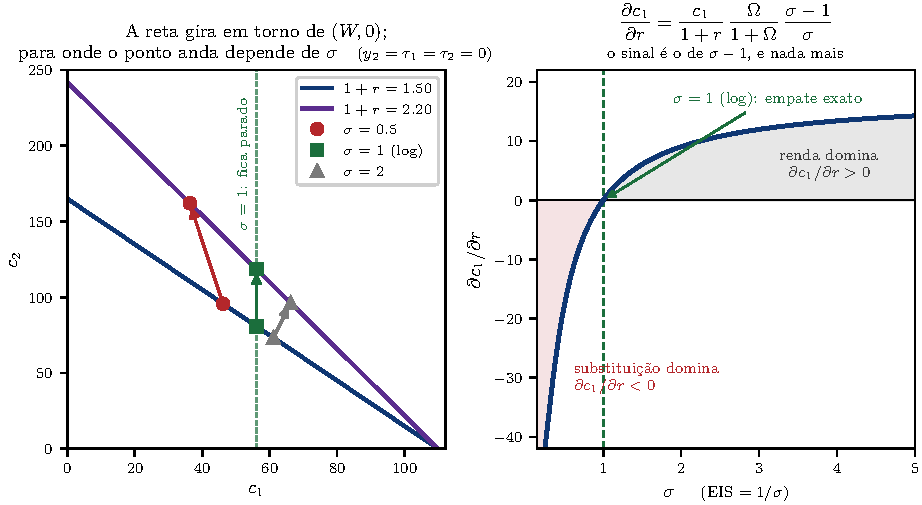
\includegraphics[width=\textwidth]{fig/fig_l3q1_sigma.pdf}
\caption{\small \textbf{Esquerda:} com $y_2=0$ a reta orçamentária gira em torno de
$(W,0)$ --- o ponto $c_1=W$, $c_2=0$ é acessível a qualquer juro. As três setas mostram
para onde o ótimo migra quando $r$ sobe de $0{,}50$ para $1{,}20$: para a esquerda se
$\sigma=0{,}5$, verticalmente se $\sigma=1$, para a direita se $\sigma=2$.
\textbf{Direita:} a derivada como função de $\sigma$, cruzando zero exatamente em
$\sigma=1$.}
\end{figure}

\intuicao{A dica do enunciado (``o que $\sigma$ significa para a importância relativa dos
efeitos renda e substituição'') aponta para um fato que é fácil de recitar e difícil de
sentir: \textbf{$\sigma$ e a EIS são o mesmo parâmetro lido de dois lados}. Um $\sigma$
alto significa utilidade marginal que despenca rápido, logo forte aversão a perfis
desiguais de consumo, logo \emph{pouca} disposição a substituir entre períodos --- EIS
baixa. O efeito substituição é fraco justamente porque a curvatura é alta.

O efeito renda, por sua vez, existe aqui porque com $y_2=0$ o consumidor é
\textbf{necessariamente poupador} ($a=W-c_1>0$): ele é credor líquido, e juro maior é
notícia boa. Se ele fosse devedor, o efeito renda mudaria de sinal e passaria a reforçar
a substituição --- é exatamente o que Kurlat mostra na p.\ 110, e é por isso que a resposta
para um tomador de empréstimo seria inequívoca.

A moral prática, que reaparece na Aula 6 e no AD-AS: \textbf{a resposta da poupança
agregada ao juro é uma questão empírica, não teórica}. Estimativas usuais de EIS ficam
entre $0{,}5$ e $1$, isto é, $\sigma$ entre $1$ e $2$ --- ou seja, perto do empate. É por
isso que modelos macro frequentemente adotam o log: não apenas por conveniência algébrica,
mas porque o caso-limite é defensável.}

\refbib{Kurlat (2020), §6.2 ``The Effect of Interest Rates'' (pp.\ 108--111); a
decomposição de Hicks está na p.\ 110, com a nota de rodapé 7 contrastando-a com Slutsky.
O Exercício 6.3 do livro (p.\ 122) é o caso-limite deste item com $c_1=y_1$, $c_2=y_2$.}

\begin{tcolorbox}[rubricbox]
\small
\begin{itemize}[topsep=2pt]
\item Dar a derivada correta mas não discutir o sinal em função de $\sigma$: máx.\ 0,4 ---
      o enunciado é explícito (``How does the answer depend on $\sigma$?'').
\item Trocar $\sigma$ por EIS na interpretação (dizer que $\sigma$ alto $\Rightarrow$ muita
      substituição): erro conceitual, teto de 0,5 no item mesmo com álgebra correta.
\item Afirmar que juro maior sempre aumenta a poupança: máx.\ 0,3.
\item Não identificar o caso log como o divisor de águas: $-0{,}3$.
\item Não notar que o consumidor aqui é obrigatoriamente poupador (e por isso o efeito
      renda tem o sinal que tem): $-0{,}2$.
\end{itemize}
\textbf{Bônus:} escrever a resposta em elasticidade e observar que ela é o produto de
$(1-\text{EIS})$ pela fração da riqueza destinada ao futuro.
\end{tcolorbox}

%---------------------------------------------------------------- (d)
\subsection*{(d) Caso geral: o que a tributação faz com $c_1$, $c_2$ e $a$}

\passo{A observação que dispensa quase toda a conta.}
Volte ao item (a). Os impostos aparecem em \emph{um único lugar}: dentro de $W$. E a razão
$\theta=c_2/c_1$ não depende deles. Logo, antes de derivar qualquer coisa já sabemos que
\textbf{um imposto \emph{lump-sum} é um puro efeito-riqueza}: ele empurra o consumidor para
um ponto mais baixo da \emph{mesma} reta de expansão, sem mudar a inclinação da restrição.
Geometricamente, a reta orçamentária sofre um \textbf{deslocamento paralelo} para dentro.

\passo{As seis derivadas.}
Com $c_1=\frac{W}{1+\Omega}$, $c_2=\theta c_1$ e $a=a_0+y_1-\tau_1-c_1$:

\begin{center}
\small
\renewcommand{\arraystretch}{1.6}
\begin{tabular}{@{}lccl@{}}
\toprule
& \textbf{Imposto hoje} ($\tau_1$) & \textbf{Imposto amanhã} ($\tau_2$) & \textbf{Leitura} \\
\midrule
$c_1$ & $\resp{-\mathrm{PMgC}}$ & $\resp{-\dfrac{\mathrm{PMgC}}{1+r}}$
  & cai nos dois casos, e \emph{menos} que 1 por 1 \\
$c_2$ & $\resp{-\theta\,\mathrm{PMgC}}$ & $\resp{-\dfrac{\theta\,\mathrm{PMgC}}{1+r}}$
  & cai nos dois casos, na mesma proporção $\theta$ \\
$a$   & $\resp{-(1-\mathrm{PMgC})}$ & $\resp{+\dfrac{\mathrm{PMgC}}{1+r}}$
  & \textbf{o único sinal que troca} \\
\bottomrule
\end{tabular}
\end{center}

\noindent onde $\mathrm{PMgC}=\frac{1}{1+\Omega}$. Na calibração de referência
($\mathrm{PMgC}=\frac59$, $\theta=1{,}2$, $r=0{,}5$): $\frac{\partial c_1}{\partial\tau_1}
=-0{,}556$, $\frac{\partial c_1}{\partial\tau_2}=-0{,}370$,
$\frac{\partial a}{\partial\tau_1}=-0{,}444$, $\frac{\partial a}{\partial\tau_2}=+0{,}370$.

\passo{Como ler cada linha.}

\begin{itemize}
\item \textbf{Consumo cai nos dois períodos, sempre.} Qualquer imposto reduz $W$, e $W$
  financia tanto $c_1$ quanto $c_2$. Não existe imposto \emph{lump-sum} que aumente algum
  consumo neste modelo.
\item \textbf{Mas cai menos que um-a-um.} Um imposto de 1 real hoje derruba $c_1$ em
  $\mathrm{PMgC}<1$ real, não em 1 real. \textbf{O consumidor suaviza}: ele reparte o
  golpe entre os dois períodos, e o instrumento com que reparte é a poupança.
\item \textbf{A poupança absorve o resíduo.} Justamente por isso,
  $\frac{\partial a}{\partial\tau_1}=-(1-\mathrm{PMgC})$: a parcela do imposto de hoje que
  \emph{não} saiu do consumo de hoje saiu da poupança. Os dois efeitos somam exatamente 1.
\item \textbf{Um imposto futuro \emph{aumenta} a poupança.} Este é o sinal que se erra.
  Sabendo que terá de pagar $\tau_2$, o consumidor \textbf{poupa hoje para pagar amanhã}
  --- e ainda assim consome menos hoje, porque ficou mais pobre. Consumo e poupança se
  movem em direções opostas.
\item \textbf{A razão entre os dois impostos é exatamente $1+r$:}
  $\frac{\partial c_1/\partial\tau_1}{\partial c_1/\partial\tau_2}=1+r$. Um real de imposto
  hoje machuca $(1+r)$ vezes mais que um real de imposto amanhã --- porque, em valor
  presente, ele \emph{é} $(1+r)$ vezes maior. Guarde: o item (e) inteiro sai daqui.
\item \textbf{A razão $c_2/c_1$ não se move.} Para qualquer $\tau_1,\tau_2$,
  $\frac{c_2}{c_1}=\theta$. Nenhuma margem foi distorcida --- e é isso que a Questão 2(d)
  vai destruir.
\end{itemize}

\intuicao{Vale explicitar o contraste que a lista está montando. Um imposto \emph{lump-sum}
é uma quantia fixa: o consumidor não pode reduzi-la mudando de comportamento. Por isso ele
não altera nenhum \emph{preço} que o consumidor enfrente --- a taxa marginal de substituição
ótima continua igual a $1+r$, que é a taxa a que a economia realmente transforma consumo
presente em futuro. O consumidor fica mais pobre e reage como reagiria a qualquer
empobrecimento: consome menos de tudo, na proporção que a homoteticidade determina.

O que \emph{não} acontece é o consumidor ``fugir'' do imposto. Não há margem de fuga. É
exatamente essa ausência de margem de fuga que faz o \emph{lump-sum} ser eficiente --- e
que a Questão 2(d) remove.}

\refbib{Kurlat (2020), §6.2 ``Taxes and Ricardian Equivalence'' (pp.\ 113--116). O livro
faz a mesma conta com $a_0=0$; a presença de $a_0$ aqui não muda derivada nenhuma, porque
$a_0$ é aditivo em $W$.}

\begin{tcolorbox}[rubricbox]
\small
\begin{itemize}[topsep=2pt]
\item Não separar os efeitos de $\tau_1$ e de $\tau_2$: máx.\ 0,5 --- o enunciado pede os
      efeitos ``da tributação'' no plural, e o item (e) depende dessa separação.
\item Errar o sinal de $\partial a/\partial\tau_2$ (dizer que é negativo): erro conceitual,
      máx.\ 0,4 no item.
\item Afirmar que $\partial c_1/\partial\tau_1 = -1$: ignora a suavização, máx.\ 0,4.
\item Não tratar da poupança: $-0{,}3$ --- o enunciado a menciona nominalmente.
\end{itemize}
\textbf{Bônus:} notar que $\frac{\partial c_1}{\partial \tau_1}=(1+r)\frac{\partial c_1}
{\partial \tau_2}$ e que $c_2/c_1$ é invariante --- as duas observações \emph{entregam} o
item (e) de graça.
\end{tcolorbox}

%---------------------------------------------------------------- (e)
\subsection*{(e) Só o valor presente importa: equivalência ricardiana}

\passo{Parte 1 --- a demonstração, em duas linhas.}
Reescreva a riqueza separando a parte fiscal:
$$W = \underbrace{a_0+y_1+\frac{y_2}{1+r}}_{\text{não depende de imposto}}
\;-\;\underbrace{\left(\tau_1+\frac{\tau_2}{1+r}\right)}_{\textstyle \equiv\, T
\ \text{(valor presente dos impostos)}}$$
Pelo item (a), $c_1=\frac{W}{1+\Omega}$ e $c_2=\theta c_1$, e $\Omega$ e $\theta$ dependem
apenas de $(\beta,r,\sigma)$. Logo $c_1$ e $c_2$ são funções de $(\tau_1,\tau_2)$
\textbf{apenas através de $T$}. Formalmente:
$$\boxed{\;\frac{\partial c_i}{\partial\tau_1}=(1+r)\,\frac{\partial c_i}{\partial\tau_2},
\quad i=1,2
\;\Longleftrightarrow\;
\text{qualquer } (d\tau_1,d\tau_2) \text{ com } dT=0 \text{ deixa } c_1,c_2 \text{ intactos.}}$$
Note que \textbf{a demonstração não usa a forma CRRA}: ela vale para qualquer $u$ côncava,
porque o único canal pelo qual imposto entra no problema é a RIO, e na RIO ele entra só
como $T$. A CRRA serve apenas para escrever a resposta em forma fechada.

\passo{Parte 2 --- o experimento pedido: $d\tau_1=-1$, $d\tau_2=+(1+r)$.}
Primeiro, confirme que é neutro em valor presente:
$$dT = d\tau_1 + \frac{d\tau_2}{1+r} = -1 + \frac{1+r}{1+r} = -1 + 1 = \resp{0}$$
Portanto $dW=0$ e:

\begin{center}
\small
\renewcommand{\arraystretch}{1.4}
\begin{tabular}{@{}clp{8.1cm}@{}}
\toprule
\textbf{Variável} & \textbf{Efeito} & \textbf{Por quê} \\
\midrule
$c_1$ & $\resp{d c_1 = 0}$ & $W$ não mudou; a decisão de consumo não vê o \emph{timing}. \\
$c_2$ & $\resp{d c_2 = 0}$ & idem, e além disso $\theta$ não mudou. \\
$a$   & $\resp{d a = +1}$
  & $a=a_0+y_1-\tau_1-c_1 \Rightarrow da = -d\tau_1 - dc_1 = +1 - 0 = +1$. \\
\bottomrule
\end{tabular}
\end{center}

\passo{Verificação independente pela restrição do período 2.} Um bom teste de consistência:
$$dc_2 = -d\tau_2 + (1+r)\,da = -(1+r) + (1+r)\cdot 1 = 0 \quad\checkmark$$
Bate com a linha de cima, por um caminho diferente. Na calibração de referência
($\tau_1{:}\,6\to5$, $\tau_2{:}\,9\to10{,}5$): $c_1$ segue $80$, $c_2$ segue $96$,
e $a$ vai de $24$ para $25$.

\begin{tcolorbox}[theorybox, title={Resposta do item (e)}]
\small
\textbf{Não, o \emph{timing} da tributação não importa para o consumo.} O corte de imposto
de hoje é \textbf{integralmente poupado}: a poupança privada sobe exatamente 1 unidade, que
é exatamente o quanto o governo precisou tomar emprestado para financiar o corte. Consumo,
utilidade e bem-estar ficam idênticos. Isso é a \textbf{equivalência ricardiana}.

\smallskip
Contabilidade agregada: a poupança pública caiu 1, a privada subiu 1, a poupança nacional
não se moveu. O consumidor está simplesmente refazendo em casa o que o governo desfez ---
o modelo não distingue ``dívida pública'' de ``imposto futuro'', porque são a mesma coisa
com nomes diferentes.
\end{tcolorbox}

\begin{figure}[htbp]
\centering
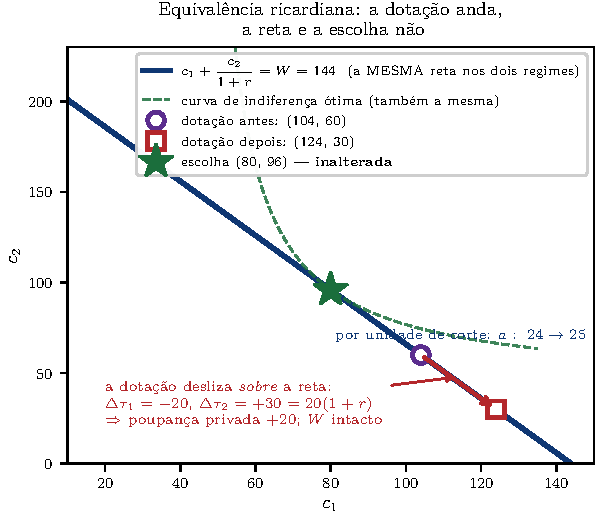
\includegraphics[width=0.72\textwidth]{fig/fig_l3q1_ricardo.pdf}
\caption{\small A troca fiscal move a \textbf{dotação} ao longo da reta orçamentária, mas
não move a reta: a dotação nova continua satisfazendo $c_1+\frac{c_2}{1+r}=W=144$. Como o
conjunto factível é o mesmo, a escolha é a mesma. A única coisa que muda é a
\emph{distância} entre dotação e escolha --- que é, precisamente, a poupança. Na figura o
deslocamento foi ampliado para $\Delta\tau_1=-20$ apenas para ficar visível; por unidade de
corte, $a$ vai de 24 para 25.}
\end{figure}

\passo{As quatro hipóteses --- e por que este item existe.}
Kurlat dedica a p.\ 115 a alertar que a equivalência é frágil. As condições que a
sustentam, e o que as quebra:

\begin{center}
\small
\begin{tabular}{@{}lp{5.3cm}p{5.6cm}@{}}
\toprule
\textbf{Hipótese} & \textbf{O que ela exige} & \textbf{Quem a quebra} \\
\midrule
\textbf{Impostos \emph{lump-sum}}
  & O imposto não muda preço relativo nenhum.
  & \textbf{Questão 2(d)} --- um imposto sobre o retorno da poupança muda. \\
\textbf{Sem restrição de crédito}
  & O consumidor pode poupar (e despoupar) livremente o valor do corte.
  & \textbf{Questão 2(c)} --- com $a\ge-b$ ativa, ele não pode. \\
\textbf{Mesmo $r$ para governo e consumidor}
  & Ambos descontam a $1+r$, senão $dT\ne0$ para um deles.
  & Prêmio de risco soberano; \emph{spread} de crédito ao consumidor. \\
\textbf{O consumidor paga o imposto futuro}
  & Ele está vivo e é ele quem paga.
  & Horizonte finito / gerações sobrepostas; migração. \\
\bottomrule
\end{tabular}
\end{center}

\begin{tcolorbox}[trapbox, title={O que a equivalência ricardiana NÃO diz}]
\small
Kurlat faz esse alerta explicitamente (p.\ 115), ``porque as pessoas às vezes entendem isso
errado''. A equivalência \textbf{não} afirma que a política fiscal é irrelevante. Ela
afirma algo muito mais estreito: \emph{dado} um caminho de gastos do governo, trocar
impostos \emph{lump-sum} de hoje por impostos \emph{lump-sum} de amanhã de mesmo valor
presente não muda o consumo. Continuam importando: o \textbf{nível} do gasto público, a
\textbf{composição} dele, e o \textbf{tipo} de imposto usado. As duas questões da lista
juntas são a demonstração disso.
\end{tcolorbox}

\refbib{Kurlat (2020), §6.2 ``Taxes and Ricardian Equivalence'' (pp.\ 113--116), com o
alerta sobre interpretações erradas na p.\ 115 e a remissão explícita ao Exercício 6.5 ---
que é a Questão 2 desta lista. Romer (2012, arquivo local), cap.\ 12, dá a versão com
horizonte infinito e gerações sobrepostas.}

\begin{tcolorbox}[rubricbox]
\small
\begin{itemize}[topsep=2pt]
\item Verificar o experimento numericamente sem \emph{demonstrar} que $\tau_1,\tau_2$
      entram só via $T$: máx.\ 0,5 --- o enunciado começa com ``Show that''.
\item Responder que $c_1$ não muda mas não dizer o que acontece com $a$: $-0{,}4$. A
      poupança é onde o ajuste inteiro acontece.
\item Concluir que ``política fiscal não tem efeito'': erro conceitual grave, máx.\ 0,4 no
      item mesmo com toda a álgebra certa.
\item Não listar nenhuma hipótese: $-0{,}3$.
\end{itemize}
\textbf{Bônus de completude:} observar que a demonstração vale para \emph{qualquer} $u$
côncava (a CRRA nunca é usada), e antecipar que a Questão 2 é o contraexemplo construído
sobre as duas primeiras hipóteses da tabela.
\end{tcolorbox}

%======================================================================
\section[Questão 2 --- As duas maneiras de quebrar Ricardo]{Questão 2 \quad As duas maneiras de quebrar o resultado da Questão 1}
%======================================================================

\begin{tcolorbox}[questionbox]
\small
Suppose a household solves a variant of the previous problem
$$\max_{\{c_1,a,c_2\}} u(c_1)+\beta u(c_2)
\qquad \text{s.t.} \quad
\begin{aligned}
c_1 + a &= y_1 - \tau_1 \\
c_2 &= y_2 - \tau_2 + (1+r)a \\
a &\ge -b
\end{aligned}$$

\smallskip
\textbf{(a)} What does the new constraint mean? What does $b$ represent?
\textbf{(b)} Give two examples of when this constraint is more likely to be binding.
\textbf{(c)} Solve for $c_1$, $c_2$ and $a$. \emph{Hint: Notice the new constraint may or
may not be binding. Consider both cases.}
\textbf{(d)} Suppose now that, rather than levying a lump-sum tax in period 2, the
government taxes the return to savings. The second-period budget constraint becomes
$$c_2 = y_2 + (1+r-\tau_2)\,a$$
Compare this tax with a lump-sum tax that raises the same revenue. Show that taxing savings
will change the ratio $\frac{c_2}{c_1}$ while a lump-sum tax does not, and explain which
margin each type of taxation distorts.
\end{tcolorbox}

\begin{tcolorbox}[theorybox, title={Duas mudanças em relação à Questão 1, e por que elas são as duas certas}]
\small
Sumiu $a_0$ (irrelevante --- era aditivo em $W$) e entrou $a\ge-b$. Nos itens (a)--(c) a
questão ataca a hipótese ``\emph{sem restrição de crédito}''; no item (d), a hipótese
``\emph{impostos lump-sum}''. São exatamente as duas primeiras linhas da tabela de
hipóteses do item 1(e) --- a Questão 2 não é um exercício novo, é o \textbf{contraexemplo
construído} da Questão 1.
\end{tcolorbox}

%---------------------------------------------------------------- 2(a)
\subsection*{(a) O que a restrição significa e o que é $b$}

\passo{Leitura direta.}
$a$ é a posição de ativos com que o domicílio termina o período 1. Quando $a>0$ ele é
credor; quando $a<0$, devedor, e $-a$ é o tamanho da dívida. A restrição
$$a \ge -b \quad\Longleftrightarrow\quad -a \le b$$
diz então: \textbf{a dívida contraída no período 1 não pode passar de $b$}. É uma
\textbf{restrição de crédito} (\emph{borrowing constraint} / \emph{credit constraint}), e
$b\ge0$ é o \textbf{limite de endividamento} --- o máximo que o sistema financeiro está
disposto a emprestar a este domicílio.

\begin{center}
\small
\begin{tabular}{@{}clp{8.4cm}@{}}
\toprule
\textbf{Valor de $b$} & \textbf{Significa} & \textbf{Leitura econômica} \\
\midrule
$b=0$ & $a\ge0$ & Nenhum crédito. O domicílio pode poupar, mas não pode se endividar
  contra renda futura. \\
$0<b<\infty$ & $a\ge-b$ & Crédito racionado. Há mercado de crédito, mas com teto. \\
$b\to\infty$ & sem restrição & Volta-se exatamente à Questão 1 (com $a_0=0$). \\
\bottomrule
\end{tabular}
\end{center}

\passo{De onde vem $b$, e o teto natural.}
A restrição não é uma preferência do domicílio: é uma \textbf{imperfeição do mercado de
crédito}. O credor não consegue verificar a renda futura, ou não consegue executar a
garantia, ou a lei protege o devedor --- e por isso raciona. Nesse sentido, $b$ mede a
\textbf{fração da renda futura que o domicílio consegue efetivamente dar como garantia}.

Há um teto acima do qual $b$ deixa de restringir coisa alguma. Como o modelo acaba no
período 2, exige-se $c_2\ge0$:
$$c_2 = y_2-\tau_2+(1+r)a \ \ge\ 0
\quad\Longleftrightarrow\quad
a \ \ge\ -\frac{y_2-\tau_2}{1+r}$$
Esse é o \textbf{limite natural de dívida}: o valor presente da renda líquida futura, isto
é, o máximo que o domicílio poderia pagar mesmo consumindo zero amanhã. Portanto:
$$\resp{b < \frac{y_2-\tau_2}{1+r}}\ \Rightarrow\ \text{a restrição é uma imposição real
do mercado};\qquad
b \ge \frac{y_2-\tau_2}{1+r}\ \Rightarrow\ \text{quem restringe é a solvência, não } b.$$

\intuicao{Repare no que a restrição \emph{não} faz. Ela não impede o domicílio de poupar
--- $a$ pode ser tão grande quanto se queira. Ela é assimétrica: morde de um lado só. Essa
assimetria é a razão de a resposta do item (c) ter dois regimes em vez de dois lados
simétricos, e é a razão econômica pela qual restrições de crédito afetam desproporcio\-nal\-mente
quem é jovem, pobre ou informal --- gente cuja renda esperada está toda no futuro.}

\refbib{Kurlat (2020), Exercício 6.5 (p.\ 122), enunciado original; §6.2, p.\ 115, onde o
texto lista as hipóteses da equivalência ricardiana e remete a este exercício como o
contraexemplo.}

%---------------------------------------------------------------- 2(b)
\subsection*{(b) Quando a restrição tende a morder}

\passo{O método certo: interrogar a fórmula, não a intuição.}
A restrição morde quando o $a$ que o domicílio \emph{escolheria sem ela} já é menor que
$-b$. Do item 1(a), com $a_0=0$:
$$a^{u} = \underbrace{\frac{\Omega}{1+\Omega}}_{>0}\,(y_1-\tau_1)
\;-\;\underbrace{\frac{1}{1+\Omega}\cdot\frac{y_2-\tau_2}{1+r}}_{>0}$$
Basta perguntar o que torna essa expressão mais negativa. Ela cai quando $y_1-\tau_1$ cai,
quando $y_2-\tau_2$ sobe, e (via $\Omega$) quando o domicílio é mais impaciente. Some-se a
isso o próprio $b$ ser baixo, e temos a lista completa.

\passo{Dois exemplos, cada um apontando para um termo diferente da fórmula.}

\begin{tcolorbox}[planbox, title={Exemplo 1 --- perfil de renda íngreme: o jovem em início de carreira}]
\small
Um residente de medicina, um estagiário, um doutorando. $y_1$ é baixo, $y_2$ é alto e
razoavelmente previsível: \textbf{o segundo termo domina o primeiro} e $a^u$ é fortemente
negativo. Ele \emph{quer} tomar emprestado contra a renda futura, e essa é a coisa
economicamente correta a fazer --- é suavização de consumo pura.

O problema é que ele é exatamente quem tem menos a oferecer como garantia: sem patrimônio,
sem histórico de crédito, e com renda futura que o banco não consegue penhorar. Logo
$b$ é pequeno \emph{ao mesmo tempo} em que $|a^u|$ é grande. As duas pontas se movem no
sentido errado simultaneamente.
\end{tcolorbox}

\begin{tcolorbox}[planbox, title={Exemplo 2 --- choque transitório negativo de renda}]
\small
Desemprego temporário, safra perdida, doença que interrompe o trabalho, fechamento
temporário de um negócio. $y_1$ despenca enquanto $y_2$ permanece --- ou seja,
\textbf{$y_1-\tau_1$ cai e a diferença toda vai para $a^u$}. O livro-texto manda suavizar:
tome emprestado hoje, pague quando a renda voltar.

Mas o credor observa a mesma queda de renda e a lê como risco. O crédito encolhe
precisamente quando é mais necessário. É por isso que restrições de crédito são
\textbf{pró-cíclicas} e amplificam recessões: elas mordem justamente no estado da natureza
em que o seguro seria mais valioso.
\end{tcolorbox}

\passo{Mais dois, para completude.}
\emph{(iii) Impaciência alta} ($\beta$ baixo, logo $\Omega$ baixo, logo $\mathrm{PMgC}$
alta): o domicílio quer antecipar consumo, e $a^u$ cai.
\emph{(iv) Imposto concentrado no presente} ($\tau_1$ alto): é uma queda de $y_1-\tau_1$
por outro nome, com o mesmo efeito do Exemplo 2 --- e é a ponte direta com o item (c).

\begin{tcolorbox}[trapbox, title={O contraexemplo que o enunciado espera que você evite}]
\small
``O domicílio é pobre'' \textbf{não é} um bom exemplo. Pobreza nos \emph{dois} períodos
reduz $y_1$ e $y_2$ juntos, e os dois termos de $a^u$ caem em direções opostas ---
o efeito líquido sobre $a^u$ é ambíguo. O que faz a restrição morder não é o nível da
renda, é a sua \textbf{inclinação no tempo}. Um exemplo bom sempre nomeia um perfil
$y_1$ baixo \emph{contra} $y_2$ alto, nunca um nível baixo.
\end{tcolorbox}

\refbib{Kurlat (2020), Exercício 6.5(d) (p.\ 122), que pede exatamente as três condições
--- $y_2-\tau_2$ alto, $y_1-\tau_1$ baixo, $b$ baixo --- e a interpretação de cada uma.}

%---------------------------------------------------------------- 2(c)
\subsection*{(c) Solução com a restrição: dois regimes, e o teste que decide qual vale}

\passo{Montagem.} Substitua as duas restrições de fluxo na objetivo, deixando o problema
em uma variável só:
$$\max_{a\,\ge\,-b}\ V(a) \equiv u(y_1-\tau_1-a) + \beta\,u\big(y_2-\tau_2+(1+r)a\big)$$
$V$ é estritamente côncava e o conjunto $[-b,\infty)$ é convexo, então as condições de
Karush--Kuhn--Tucker são necessárias e suficientes. Com multiplicador $\phi\ge0$ associado
a $a+b\ge0$:
$$\underbrace{-u'(c_1)+\beta(1+r)u'(c_2)}_{V'(a)} + \phi = 0,
\qquad \phi\ge0, \qquad \phi\,(a+b)=0$$
ou seja
$$\boxed{\;u'(c_1) = \beta(1+r)\,u'(c_2) + \phi\;}$$
\textbf{A Euler ganha um termo.} $\phi$ é o valor, em utilidade, de relaxar o limite de
crédito em uma unidade --- o preço-sombra do crédito que falta.

\passo{Caso 1 --- restrição folgada ($\phi=0$, $a>-b$).}
A Euler volta a valer com igualdade e a solução é a da Questão 1 com $a_0=0$:
$$c_1^{u} = \frac{y_1-\tau_1+\dfrac{y_2-\tau_2}{1+r}}{1+\Omega},
\qquad c_2^{u} = \theta\,c_1^{u},
\qquad a^{u} = y_1-\tau_1-c_1^{u}$$

\passo{Caso 2 --- restrição ativa ($a=-b$, $\phi>0$).}
Aqui não há o que otimizar: a escolha \emph{é} o canto. Basta ler as restrições de fluxo:
$$a = -b,\qquad c_1 = y_1-\tau_1+b,\qquad c_2 = y_2-\tau_2-(1+r)b$$
E a Euler passa a valer como \textbf{desigualdade estrita}:
$$u'(c_1) > \beta(1+r)u'(c_2)
\quad\Longleftrightarrow\quad
\resp{\frac{c_2}{c_1} < [\beta(1+r)]^{1/\sigma} = \theta}$$
Leia devagar: a utilidade marginal de hoje é \emph{alta demais} em relação à de amanhã. O
domicílio queria trazer recursos do futuro para o presente e não conseguiu. O perfil de
consumo é mais inclinado do que ele gostaria.

\passo{Qual caso vale? O teste.}
O Caso 1 é válido se e somente se $a^u\ge-b$. Equivalentemente --- e esta é a forma útil:
$$\boxed{\;\text{a restrição está \textbf{ativa}}
\iff c_1^{u} > y_1-\tau_1+b
\iff \frac{y_2-\tau_2}{1+r} > \Omega\,(y_1-\tau_1) + b\,(1+\Omega)\;}$$
A leitura do meio é a mais direta: \emph{o consumo que ele queria é maior do que o consumo
que ele consegue pagar}. As três condições do item (b) estão todas visíveis na versão da
direita.

\begin{tcolorbox}[theorybox, title={Resposta do item (c)}]
$$\resp{a\stst = \max\{\,a^{u},\ -b\,\}}, \qquad
\resp{c_1\stst = \min\{\,c_1^{u},\ y_1-\tau_1+b\,\}}, \qquad
\resp{c_2\stst = y_2-\tau_2+(1+r)\,a\stst}$$
com $c_1^u$ e $a^u$ dados pelo Caso 1. Em palavras: \emph{siga a solução irrestrita; se ela
pedir mais dívida do que $b$, pare em $-b$.}
\end{tcolorbox}

\begin{figure}[htbp]
\centering
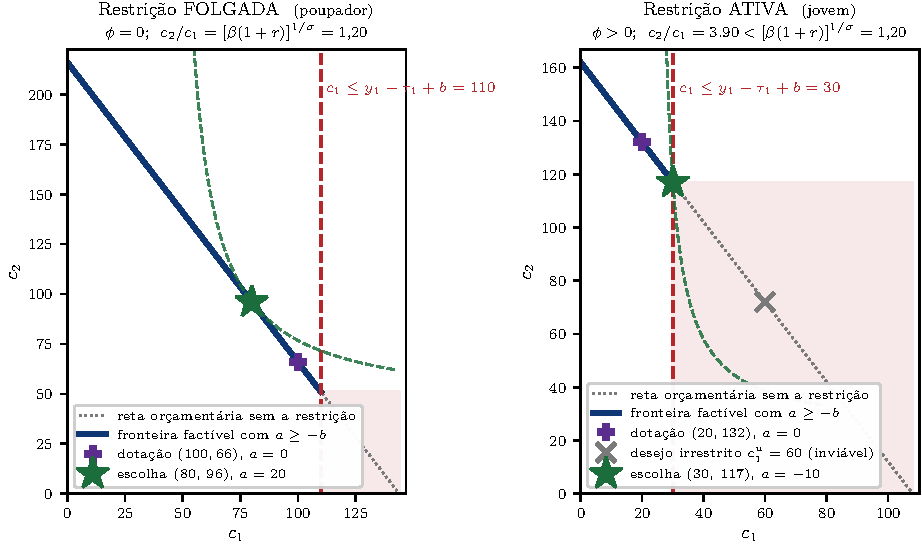
\includegraphics[width=\textwidth]{fig/fig_l3q2_restricao.pdf}
\caption{\small A restrição corta o conjunto factível por uma vertical em
$c_1=y_1-\tau_1+b$. \textbf{Esquerda:} o poupador ($y_1=100$, $y_2=66$) escolhe bem à
esquerda do corte --- a restrição existe mas não faz nada, $\phi=0$ e $c_2/c_1=1{,}20$.
\textbf{Direita:} o jovem ($y_1=20$, $y_2=132$) queria $c_1^u=60$ e para em $c_1=30$; a
tangência é impossível e o ótimo vai para o canto, com $c_2/c_1=3{,}90\gg1{,}20$ --- o
perfil é muito mais inclinado do que ele gostaria.}
\end{figure}

\passo{A consequência que a lista está construindo.}
No regime ativo, $c_1 = y_1-\tau_1+b$. Derive:
$$\frac{\partial c_1}{\partial y_1}=\resp{1},
\qquad \frac{\partial c_1}{\partial y_2}=\resp{0},
\qquad \frac{\partial c_1}{\partial \tau_1}=\resp{-1}$$
Compare com o item 1(b), onde essas derivadas eram $\mathrm{PMgC}$,
$\frac{\mathrm{PMgC}}{1+r}$ e $-\mathrm{PMgC}$. \textbf{A propensão marginal a consumir
salta para 1 e a renda futura para de importar.} O domicílio restrito volta a ser
``mão-a-boca'': o consumo dele é descrito pela função consumo \emph{keynesiana} do §6.1,
não pela renda permanente. A visão que o modelo tinha rejeitado no item 1(b) reaparece
--- não como teoria alternativa, mas como o que acontece com um subconjunto identificável
de domicílios.

\begin{tcolorbox}[trapbox, title={E aqui morre a equivalência ricardiana}]
\small
Refaça o experimento do item 1(e) --- cortar $\tau_1$ em $\Delta$ e elevar $\tau_2$ em
$\Delta(1+r)$, valor presente inalterado --- para os dois regimes:

\smallskip
\begin{center}
\small
\begin{tabular}{@{}lcp{7.2cm}@{}}
\toprule
\textbf{Regime} & \textbf{$\Delta c_1$} & \textbf{Por quê} \\
\midrule
Folgado & $0$ & O domicílio poupa o corte inteiro (item 1e). \\
\textbf{Ativo} & $\resp{+\Delta}$
  & $c_1=y_1-\tau_1+b$ sobe um-a-um com o corte. Ele \textbf{não pode} poupar o dinheiro:
    ele já queria estar consumindo mais e estava impedido. O estímulo é integralmente
    gasto. \\
\bottomrule
\end{tabular}
\end{center}

\smallskip
Na calibração de referência, com $\Delta=5$: o poupador não muda o consumo (e sua poupança
vai de 20 para 25); o jovem restrito passa de $c_1=30$ para $c_1=35$. \textbf{Este é o
argumento inteiro a favor de estímulos fiscais direcionados}: transferências valem mais
quando vão para quem está restrito, e a magnitude do multiplicador depende de \emph{qual
fração} da população está no regime ativo.
\end{tcolorbox}

\refbib{Kurlat (2020), Exercício 6.5 (p.\ 122) --- a dica do enunciado do professor é
palavra por palavra a do livro. Para o alerta de que a Euler vira desigualdade, veja
\texttt{rules/04\_consumo\_poupanca.md}, seção ``Armadilhas frequentes'', item 6.}

\begin{tcolorbox}[rubricbox]
\small
\begin{itemize}[topsep=2pt]
\item Resolver só o caso folgado (repetir a Questão 1): máx.\ 0,3 do item --- a dica do
      enunciado é explícita sobre os dois casos.
\item Escrever a Euler com igualdade no caso ativo: erro conceitual, máx.\ 0,4 no item.
\item Dar os dois casos mas não estabelecer \emph{qual} vale (o teste do limiar): $-0{,}3$
      --- o enunciado diz ``Then figure out whether or not it will be binding''.
\item Não notar que $\mathrm{PMgC}=1$ no regime ativo: $-0{,}2$; é a consequência
      econômica do item.
\end{itemize}
\textbf{Bônus de completude:} fechar o ciclo com o item 1(e), mostrando que o mesmo
estímulo fiscal tem efeito 0 num regime e $+\Delta$ no outro. É a razão de a Questão 2
existir.
\end{tcolorbox}

%---------------------------------------------------------------- 2(d)
\subsection*{(d) Imposto sobre a poupança contra \emph{lump-sum} de mesma receita}

\passo{O que exatamente está sendo tributado.}
A restrição do período 2 vira $c_2 = y_2 + (1+r-\tau_2)a$, isto é, o domicílio que poupa
$a$ paga $\tau_2 a$ ao governo. Defina o \textbf{retorno bruto líquido de imposto}
$$\Rt \equiv 1+r-\tau_2 .$$
Duas observações de leitura. Primeira: escrevendo $\tau_2=\tilde\tau\,r$, a arrecadação
vira $\tilde\tau\,r\,a$ --- um imposto de alíquota $\tilde\tau$ sobre a \emph{renda de
juros}, que é a forma do Exercício 6.6 do Kurlat. As duas formulações são a mesma coisa.
Segunda: como escrito, o imposto incidiria também sobre $a<0$ (subsidiando devedores);
seguindo o Kurlat, tratamos o caso relevante do \textbf{poupador}, $a>0$, e comentamos o
bico ao final.

\passo{Passo 1 --- a nova Euler.}
O trade-off mudou: abrir mão de uma unidade de $c_1$ agora rende $\Rt$ unidades de $c_2$,
não $(1+r)$. Maximizando $u(y_1-a)+\beta u(y_2+\Rt a)$:
$$-u'(c_1)+\beta\Rt\,u'(c_2)=0
\quad\Longrightarrow\quad
\boxed{\;\frac{c_2}{c_1} = \big[\beta(1+r-\tau_2)\big]^{1/\sigma}\;}$$

\passo{Passo 2 --- a comparação que o enunciado pede.}

\begin{center}
\small
\renewcommand{\arraystretch}{1.5}
\begin{tabular}{@{}lccc@{}}
\toprule
& \textbf{Sem imposto} & \textbf{\emph{Lump-sum} $T$} & \textbf{Imposto sobre a poupança $\tau_2$} \\
\midrule
Restrição intertemporal
  & $c_1+\frac{c_2}{1+r}=y_1+\frac{y_2}{1+r}$
  & $c_1+\frac{c_2}{1+r}=y_1+\frac{y_2-T}{1+r}$
  & $c_1+\frac{c_2}{\Rt}=y_1+\frac{y_2}{\Rt}$ \\
Inclinação da reta
  & $-(1+r)$ & $-(1+r)$ \ \resp{(igual)} & $-\Rt$ \ \resp{(mais plana)} \\
Efeito geométrico
  & --- & \resp{translação paralela} & \resp{rotação em torno de $(y_1,y_2)$} \\
Razão $c_2/c_1$
  & $[\beta(1+r)]^{1/\sigma}$
  & $[\beta(1+r)]^{1/\sigma}$ \ \resp{(inalterada)}
  & $[\beta\Rt]^{1/\sigma}$ \ \resp{(menor)} \\
\bottomrule
\end{tabular}
\end{center}

\passo{Passo 3 --- a demonstração pedida, nas duas metades.}

\emph{Metade 1: o \emph{lump-sum} não mexe na razão.} No item 1(d) já vimos que
$\tau_1$ e $\tau_2$ \emph{lump-sum} entram na solução apenas via $W$, e que
$c_2/c_1=\theta$ depende só de $(\beta,r,\sigma)$. Logo
$\frac{\partial (c_2/c_1)}{\partial T}=0$ para qualquer $T$. \checkmark

\emph{Metade 2: o imposto sobre a poupança mexe.} Como $\tau_2>0$ implica $\Rt<1+r$, e
$x\mapsto(\beta x)^{1/\sigma}$ é estritamente crescente para todo $\sigma>0$:
$$\big[\beta\Rt\big]^{1/\sigma} < \big[\beta(1+r)\big]^{1/\sigma}
\quad\Longrightarrow\quad
\resp{\left(\frac{c_2}{c_1}\right)^{\text{poupança}} < \left(\frac{c_2}{c_1}\right)^{\text{lump-sum}}}$$
\textbf{para todo $\sigma>0$}, sem exceção. Na calibração de referência ($y_1=100$,
$y_2=66$, $r=0{,}5$, $\tau_2=0{,}2$, $\sigma=2$): a razão cai de $\sqrt{1{,}44}=1{,}200$
para $\sqrt{0{,}96\times1{,}3}=1{,}117$.

\passo{Passo 4 --- ``mesma receita'': fixando a comparação corretamente.}
A comparação só é honesta se os dois impostos arrecadarem o mesmo. Seja $a^S$ a poupança
escolhida sob o imposto sobre a poupança; a receita é $T = \tau_2 a^S$, e é esse $T$ que se
cobra no regime \emph{lump-sum}. Com os números: $a^S=18{,}91$, logo
$T=0{,}2\times18{,}91=3{,}78$.

\begin{center}
\small
\begin{tabular}{@{}lccccc@{}}
\toprule
\textbf{Regime} & $c_1$ & $c_2$ & $a$ & $c_2/c_1$ & $U$ \\
\midrule
Sem imposto & $80{,}00$ & $96{,}00$ & $20{,}00$ & $1{,}2000$ & $-0{,}022500$ \\
Imposto sobre a poupança, $\tau_2=0{,}2$ & $81{,}09$ & $90{,}59$ & $18{,}91$ & \resp{$1{,}1171$} & $-0{,}0229300$ \\
\emph{Lump-sum} $T=3{,}78$ (mesma receita) & $78{,}60$ & $94{,}32$ & $21{,}40$ & \resp{$1{,}2000$} & \resp{$-0{,}0229010$} \\
\bottomrule
\end{tabular}
\end{center}

\passo{Passo 5 --- por que o \emph{lump-sum} é estritamente melhor (o argumento de dominância).}
Este é o passo elegante, e não precisa de nenhum número. Tome o plano escolhido sob o
imposto sobre a poupança, $(c_1^S, c_2^S)$, com $c_1^S=y_1-a^S$ e
$c_2^S=y_2+(1+r)a^S-\tau_2 a^S$. Precifique-o à taxa \emph{de mercado} $1+r$:
$$c_1^S+\frac{c_2^S}{1+r}
= y_1-a^S+\frac{y_2+(1+r)a^S-\tau_2 a^S}{1+r}
= y_1+\frac{y_2}{1+r}-\frac{\tau_2 a^S}{1+r}
= y_1+\frac{y_2-T}{1+r}$$
usando $T=\tau_2 a^S$. Mas o lado direito é \emph{exatamente} a restrição orçamentária do
regime \emph{lump-sum}. Ou seja:

\begin{tcolorbox}[theorybox, title={O argumento em uma frase}]
\small
Sob o imposto \emph{lump-sum} de mesma receita, o plano $(c_1^S,c_2^S)$ era
\textbf{factível} --- e o domicílio, podendo escolhê-lo, \textbf{escolheu outro}. Logo o
ótimo com \emph{lump-sum} é estritamente preferido:
$U^{\text{lump-sum}} > U^{\text{poupança}}$, com a \textbf{mesma arrecadação}. A diferença
é \textbf{peso morto} (\emph{deadweight loss}, excesso de gravame).
\end{tcolorbox}

Quantificando: o \emph{lump-sum} que deixaria o domicílio exatamente tão bem quanto o
imposto sobre a poupança é $T^{\ast}=4{,}05$, contra $T=3{,}78$ efetivamente arrecadados.
O peso morto é $T^{\ast}-T=\resp{0{,}27}$, ou \resp{$7{,}1\%$ da receita} --- o governo
poderia ter arrecadado 7\% a mais sem piorar em nada a situação do domicílio, bastando
mudar o \emph{instrumento}.

\begin{figure}[htbp]
\centering
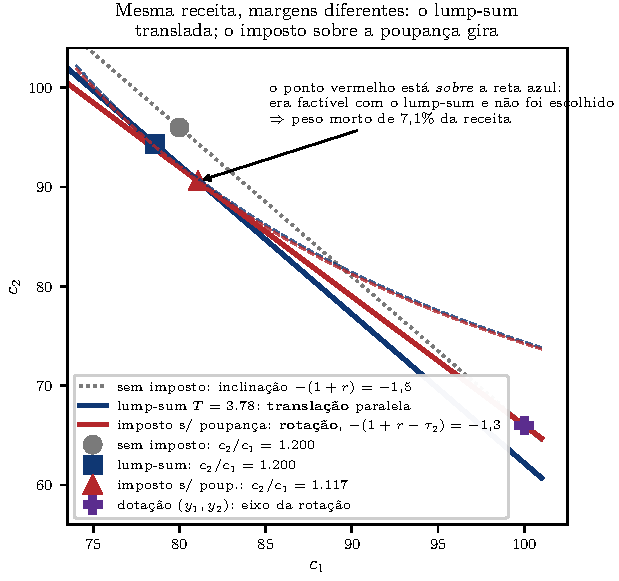
\includegraphics[width=0.74\textwidth]{fig/fig_l3q2_imposto.pdf}
\caption{\small As duas geometrias. O \emph{lump-sum} \textbf{translada} a reta
paralelamente (a inclinação segue $-1{,}5$), então o ponto de tangência anda ao longo da
mesma reta de expansão e a razão $c_2/c_1$ não muda. O imposto sobre a poupança
\textbf{gira} a reta em torno da dotação $(y_1,y_2)$ --- ponto sempre factível, pois
corresponde a $a=0$ e portanto a imposto zero --- deixando-a mais plana. O ponto vermelho
cai \emph{sobre} a reta azul: era factível no regime \emph{lump-sum} e não foi escolhido.}
\end{figure}

\passo{Passo 6 --- qual margem cada imposto distorce.}

\begin{center}
\small
\renewcommand{\arraystretch}{1.4}
\begin{tabular}{@{}lp{5.0cm}p{6.4cm}@{}}
\toprule
& \textbf{\emph{Lump-sum}} & \textbf{Imposto sobre a poupança} \\
\midrule
\textbf{Margem distorcida}
  & \resp{Nenhuma.}
  & \resp{A margem \textbf{intertemporal}} --- a escolha entre consumir hoje e consumir amanhã. \\
\textbf{O que acontece com a TMS}
  & Segue $\dfrac{u'(c_1)}{\beta u'(c_2)}=1+r$: igual à taxa a que a economia
    \emph{de fato} transforma consumo presente em futuro.
  & Passa a $\dfrac{u'(c_1)}{\beta u'(c_2)}=1+r-\tau_2 < 1+r$: abre-se uma
    \textbf{cunha} de tamanho exatamente $\tau_2$ entre o retorno privado e o social. \\
\textbf{Consequência}
  & Puro efeito-riqueza. O domicílio fica mais pobre e reduz os dois consumos na proporção
    $\theta$. Sem perda de eficiência.
  & Efeito-riqueza \emph{mais} efeito-substituição. O perfil de consumo é inclinado
    artificialmente para o presente e há perda de eficiência. \\
\textbf{Por que é assim}
  & O imposto é uma quantia fixa: não há comportamento que o reduza, logo não há
    comportamento a distorcer.
  & O imposto depende de $a$, que é escolha. Poupar menos é uma \textbf{margem de fuga} ---
    e é exatamente por poder fugir que o domicílio distorce sua decisão. \\
\bottomrule
\end{tabular}
\end{center}

\begin{tcolorbox}[trapbox, title={O que NÃO se pode concluir: o imposto sobre a poupança não necessariamente reduz a poupança}]
\small
Tentador dizer ``taxar a poupança faz poupar menos''. Mas $\tau_2$ faz duas coisas ao mesmo
tempo, e elas puxam em sentidos contrários --- é o mesmo cabo de guerra do item 1(c), agora
com $y_2>0$: \textbf{substituição} (poupar rende menos $\Rightarrow$ poupe menos) e
\textbf{riqueza} (a renda futura $y_2$ passa a ser descontada a $\Rt<1+r$, logo vale mais
em valor presente $\Rightarrow$ consuma mais hoje, mas também: para atingir um dado $c_2$ é
preciso poupar mais). O saldo depende de $\sigma$:

\smallskip
\begin{center}
\small
\begin{tabular}{@{}ccccc@{}}
\toprule
$\sigma$ & $a$ sem imposto & $a$ com $\tau_2$ & variação & $c_2/c_1$ (sem $\to$ com) \\
\midrule
$0{,}5$ & $39{,}56$ & $31{,}41$ & $-8{,}15$ & $2{,}074 \to 1{,}558$ \\
$1{,}0$ & $26{,}53$ & $23{,}08$ & $-3{,}45$ & $1{,}440 \to 1{,}248$ \\
$2{,}0$ & $20{,}00$ & $18{,}91$ & $-1{,}09$ & $1{,}200 \to 1{,}117$ \\
$4{,}0$ & $16{,}78$ & $16{,}84$ & \resp{$+0{,}06$} & $1{,}095 \to 1{,}057$ \\
\bottomrule
\end{tabular}
\end{center}

\smallskip
Com $\sigma=4$ a poupança \textbf{sobe}. Mas repare na última coluna: a razão $c_2/c_1$
cai em \emph{todas} as linhas, sem exceção. É por isso que o enunciado pede que você mostre
o efeito sobre \textbf{a razão}, e não sobre a poupança --- a razão é o que a Euler
determina sem ambiguidade, e é onde a distorção é visível.
\end{tcolorbox}

\intuicao{O resultado geral por trás deste item: para uma dada receita, \textbf{impostos
que incidem sobre margens de escolha geram peso morto; impostos que incidem sobre quantias
fixas não}. Se o \emph{lump-sum} é estritamente melhor, por que governos não o usam? Porque
ele é regressivo por construção --- a mesma quantia fixa para todos --- e porque a
capacidade de pagar não é observável sem condicionar em alguma escolha (renda, consumo,
patrimônio), e no instante em que se condiciona, cria-se a margem. O modelo de dois períodos
não tem heterogeneidade nem redistribuição, então nele o \emph{lump-sum} vence sempre; a
teoria da tributação ótima é, em boa medida, o estudo do que sobra desse resultado quando
se acrescenta desigualdade.

Uma última observação sobre o bico. Na versão do Kurlat, o devedor não paga o imposto, então
a reta orçamentária tem \textbf{inclinação $-(1+r)$ à direita da dotação e $-\Rt$ à esquerda}
--- um vinco em $(y_1,y_2)$. A consequência: para um domicílio próximo de $a=0$, um imposto
sobre a poupança pode não mudar decisão nenhuma (ele fica \emph{no} vinco), que é
exatamente o caso (iii) do Exercício 6.6(b).}

\refbib{Kurlat (2020), Exercício 6.6 (pp.\ 122--123) para o enunciado original com imposto
sobre a renda de juros; §6.2, pp.\ 108--111, para a geometria da rotação da reta ---
matematicamente, tributar a poupança e reduzir $r$ são o mesmo movimento visto de dois
ângulos.}

\begin{tcolorbox}[rubricbox]
\small
\begin{itemize}[topsep=2pt]
\item Mostrar que a razão muda mas não fixar a comparação de \emph{mesma receita}
      ($T=\tau_2 a^S$): $-0{,}3$; o enunciado exige a comparação.
\item Não identificar a margem distorcida como a \textbf{intertemporal}, ou não dizer que o
      \emph{lump-sum} não distorce nenhuma: máx.\ 0,4 no item --- é a pergunta final e
      explícita do enunciado.
\item Afirmar que o imposto sobre a poupança necessariamente reduz $a$: erro conceitual,
      máx.\ 0,5 no item.
\item Confundir rotação com translação (ou errar o ponto em torno do qual a reta gira):
      $-0{,}3$.
\item Não mostrar que $[\beta\Rt]^{1/\sigma}<[\beta(1+r)]^{1/\sigma}$ vale para todo
      $\sigma$: $-0{,}2$; sem isso o resultado parece depender da calibração.
\end{itemize}
\textbf{Bônus de completude:} o argumento de dominância do Passo 5 (``era factível e não foi
escolhido''), que estabelece o peso morto sem calcular nada, e a observação sobre o vinco
em $(y_1,y_2)$ na versão assimétrica do Kurlat.
\end{tcolorbox}

%======================================================================
\section*{Síntese --- o fio que liga as duas questões}
\addcontentsline{toc}{section}{Síntese}
%======================================================================

\begin{tcolorbox}[theorybox, title={O que a Lista 3 está realmente testando}]
\small
A lista tem uma arquitetura, e vale enxergá-la antes da prova: \textbf{a Questão 1 constrói
um resultado forte, e a Questão 2 o desmonta de duas maneiras diferentes} --- cada uma
atacando uma hipótese distinta, e cada uma com uma consequência de política distinta.

\smallskip
\begin{center}
\small
\renewcommand{\arraystretch}{1.35}
\begin{tabular}{@{}lp{4.3cm}p{4.5cm}p{4.0cm}@{}}
\toprule
& \textbf{Questão 1} & \textbf{Questão 2(a--c)} & \textbf{Questão 2(d)} \\
\midrule
\textbf{Hipótese em jogo}
 & Todas valem
 & Cai ``sem restrição de crédito''
 & Cai ``impostos \emph{lump-sum}'' \\
\textbf{O que acontece com $\mathrm{PMgC}$}
 & $\frac{1}{1+\Omega}<1$
 & \textbf{salta para 1}
 & segue $<1$ \\
\textbf{O que acontece com $c_2/c_1$}
 & $=\theta$, imune a imposto
 & $<\theta$ (Euler vira desigualdade)
 & \textbf{$<\theta$} (a cunha $\tau_2$) \\
\textbf{Geometria}
 & reta transladada
 & reta \textbf{cortada} por uma vertical
 & reta \textbf{girada} em torno da dotação \\
\textbf{Ricardo}
 & vale
 & morre
 & morre \\
\textbf{Consequência de política}
 & \emph{timing} é irrelevante
 & estímulo direcionado \textbf{funciona}
 & instrumento importa: há peso morto \\
\bottomrule
\end{tabular}
\end{center}

\smallskip
Os três mecanismos são independentes e as três colunas têm respostas diferentes. Se você
sair da lista sabendo preencher essa tabela de memória, sabe a Aula 4.
\end{tcolorbox}

\begin{tcolorbox}[trapbox, title={As três armadilhas mais caras da lista}]
\small
\begin{enumerate}[label=(\roman*)]
\item Em 1(c), trocar $\sigma$ pela EIS $1/\sigma$ na interpretação. A álgebra pode estar
inteira certa e a resposta econômica sai invertida.
\item Em 1(e), concluir que ``política fiscal não importa''. Kurlat alerta contra isso
nominalmente (p.\ 115) e a própria Questão 2 é a refutação.
\item Em 2(c), escrever a equação de Euler com igualdade no caso em que a restrição está
ativa. Além de invalidar o item, esse erro destrói a ponte com 1(e), que é a razão de a
questão existir.
\end{enumerate}
Somadas, essas três valem perto de 2,5 pontos.
\end{tcolorbox}

\begin{tcolorbox}[planbox, title={A frase que resume a lista}]
\small
\textbf{O consumo segue a riqueza, não a renda --- desde que o consumidor consiga chegar
até a sua riqueza, e desde que o governo não cobre o pedágio na porta.} A Questão 1 prova
a primeira metade da frase; os itens (a)--(c) da Questão 2 tratam da primeira ressalva; o
item (d), da segunda.
\end{tcolorbox}

%======================================================================
\section*{Apêndice \quad Código}
\addcontentsline{toc}{section}{Apêndice --- Código}
%======================================================================

Os scripts estão em \texttt{Resolucao/lista3\_codigo/} e rodam com \texttt{numpy},
\texttt{scipy} e \texttt{matplotlib} (sem dados externos --- a Lista 3 é toda analítica).
Cada resultado é conferido por um caminho independente do que produziu a fórmula.

\begin{center}
\small
\begin{tabular}{llp{7.0cm}}
\toprule
\textbf{Arquivo} & \textbf{Questão} & \textbf{O que faz} \\
\midrule
\texttt{modelo.py} & --- & Núcleo: $\Omega$, $\theta$, $W$, forma fechada, versão com
  restrição de crédito (KKT) e versão com imposto sobre a poupança. Tudo o mais importa
  daqui. \\
\texttt{l3q1\_consumo.py} & 1 & Itens (a)--(e). Confere a forma fechada contra otimização
  numérica direta, cada derivada contra diferenças centrais, e verifica que a RIO fecha e
  que o resíduo da Euler é nulo. Testa (e) para quatro valores de $\sigma$. \\
\texttt{l3q2\_restricao.py} & 2 & Itens (c)--(d). Resolve as KKT em quatro casos e confere
  contra otimização restrita; localiza o $b\stst$ que separa os regimes; demonstra
  numericamente que o plano do regime distorcido está \emph{sobre} a reta \emph{lump-sum};
  calcula o peso morto por equivalência de utilidade. \\
\texttt{l3\_figuras.py} & 1, 2 & Gera as quatro figuras. \\
\texttt{estilo\_mpl.py} & --- & Backend \texttt{pgf} (texto das figuras em fontes Type 1) e
  largura casada com a do texto, para inclusão em escala 1:1. \\
\bottomrule
\end{tabular}
\end{center}

\passo{Reprodução.}

\begin{tcolorbox}[colback=gray!7, colframe=gray!50, arc=2pt, boxrule=0.4pt]
\footnotesize
\begin{verbatim}
python l3q1_consumo.py     # itens (a)-(e) da Questao 1, com verificacoes
python l3q2_restricao.py   # itens (c)-(d) da Questao 2, com verificacoes
python l3_figuras.py       # as 4 figuras -> Resolucao/fig/
\end{verbatim}
\end{tcolorbox}

Todos os \texttt{assert} passam. Onde aparece \checkmark\ no texto, o resultado foi
confirmado por um segundo caminho independente.

\end{document}
